
% They just report mass flows
% or are proprietary and super long running

\begin{frame}[ctb!]
  \frametitle{Top Level Fuel Cycle Simulators}
  % most only report mass flows.
  \begin{figure}[htbp!]
    \begin{center}
      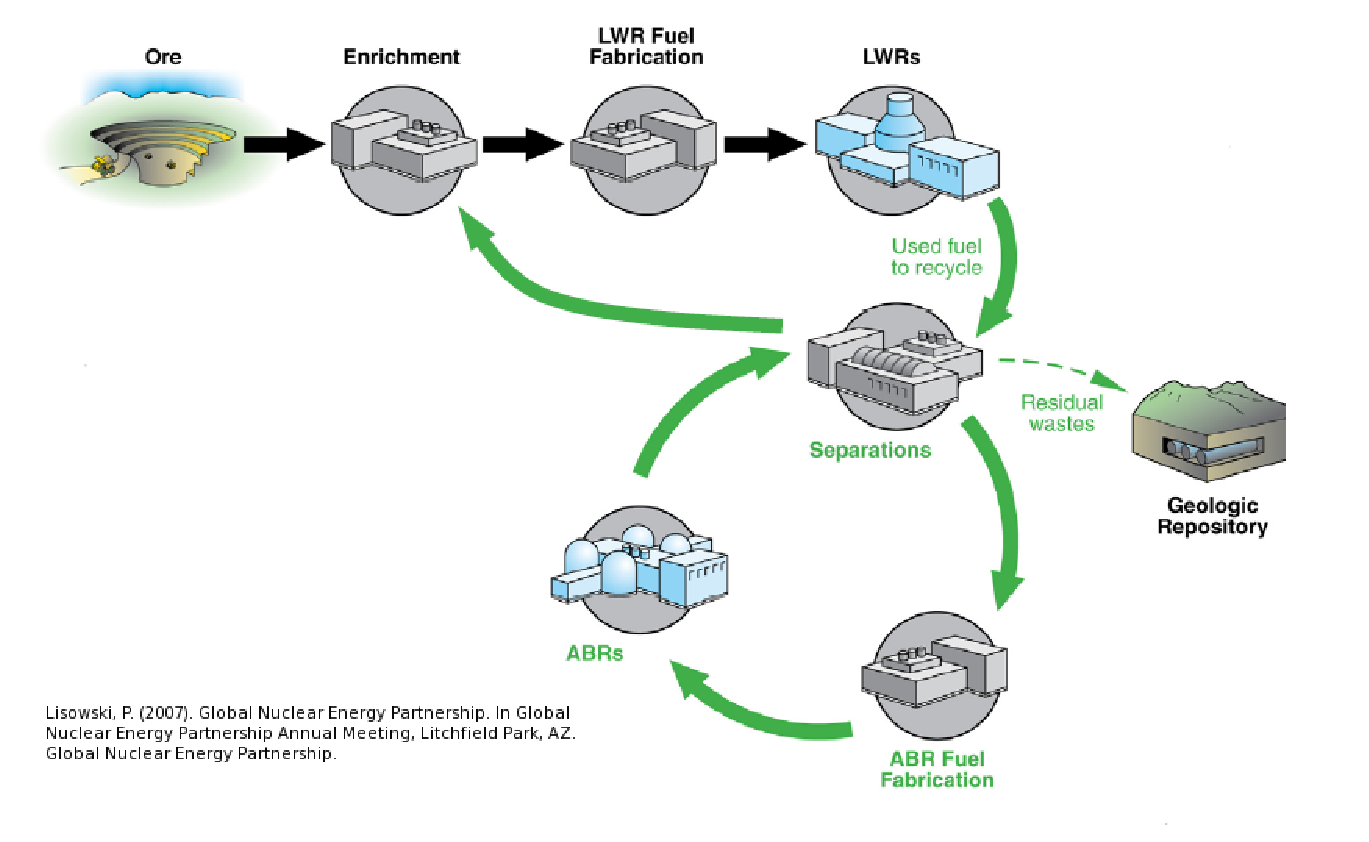
\includegraphics[height=4cm]{simulations.eps}
    \end{center}
    \caption{Top level simulators are intended to model the collective 
    behavior of various fuel cycle decisions and 
    strategies \cite{lisowski_global_2007}.}
    \label{fig:simulation}
  \end{figure}
\end{frame}

\begin{frame}[ctb!]
  \frametitle{Need For an Integrated Repository Model}
  % Incorporates disposal system decisions into metrics information
  % Captures Feedbacks
  Current fuel cycle simulators neglect disposal system decisions and 
  repository behavior. Most report masses and mass indexed metrics such 
  as radiotoxicity, both meaningless without release pathway analysis
  and not informative for disposal system options.

  %        File: systools_tab.tex
%     Created: Mon Aug 29 09:00 AM 2011 C
% Last Change: Mon Aug 29 09:00 AM 2011 C
%
\begin{table}
  \centering
  \footnotesize{
  \begin{tabular}{|l|l|c|c|c|}
    \multicolumn{5}{c}{\textbf{Repository Capabilities within Systems Analysis Tools}}\\
    \hline
    Tool & Institution & Fuel Disposition & Radionuclide Transport & Heat Transport  \\
    \hline
    NUWASTE\cite{abkowitz_nuclear_2010} & NWTRB & yes & no & no \\
    VISION \cite{yacout_vision_2006} & INL   & yes & no & YMR only \\
    DANESS \cite{van_den_durpel_daness:_2006} & ANL   & no & no & no \\
    COSI   \cite{boucher_international_2010} & CEA   & yes & no & yes \\
    NFCSim \cite{schneider_nfcsim_2004} & LANL  & no & no & no \\
    CAFCA  \cite{guerin_benchmark_2009} & MIT   & no & no & no \\
    ORION  \cite{guerin_benchmark_2009} & BNL   & no & no & no \\
    TSM    \cite{turner_discrete_2010} & OCRWM & yes & no & YMR only \\
    \hline
  \end{tabular}
  \caption[System Tools]{System tools are lacking in radionuclide transport and  
  heat transport calculations in generic geolgies.}
  \label{tab:systools}
  }
\end{table}




\end{frame}

